\subsubsection{\texttt{RN-2}: aspecto visual de la aplicación web y coherencia entre interfaces}
\label{subsec:rn2}

El diseño de la interfaz de usuario de la nueva aplicación web aspira a ser coherente con la estética que venía empleándose en la extensión para Visual Studio Code, pretendiendo formar un entono familiar para quien ya utilizase la extensión de \textit{VSCode4Teaching} para Visual Studio Code.

La \referenciaFigura{fig:reqn2-1} muestra los dos \textit{dashboards} para el seguimiento del progreso de los ejercicios existentes: el de la extensión (abajo), que no se ha visto modificado y ya existía; y el de la aplicación web (arriba), que, inspirado en el diseño anterior, refleja la misma información haciendo uso de elementos gráficos de similar índole, ya que emplea el mismo esquema cromático y los mismos iconos informativos.

Esto también se observa en la \referenciaFigura{fig:reqn2-2}, que permite observar que los iconos empleados para la distinción de las tipologías de ejercicios son los mismos y que los dispuestos para las acciones de gestión de matriculados, compartición y adición de ejercicios son muy similares, potenciando la familiaridad del entorno a los usuarios.

\begin{figure}[!p]
    \centering
    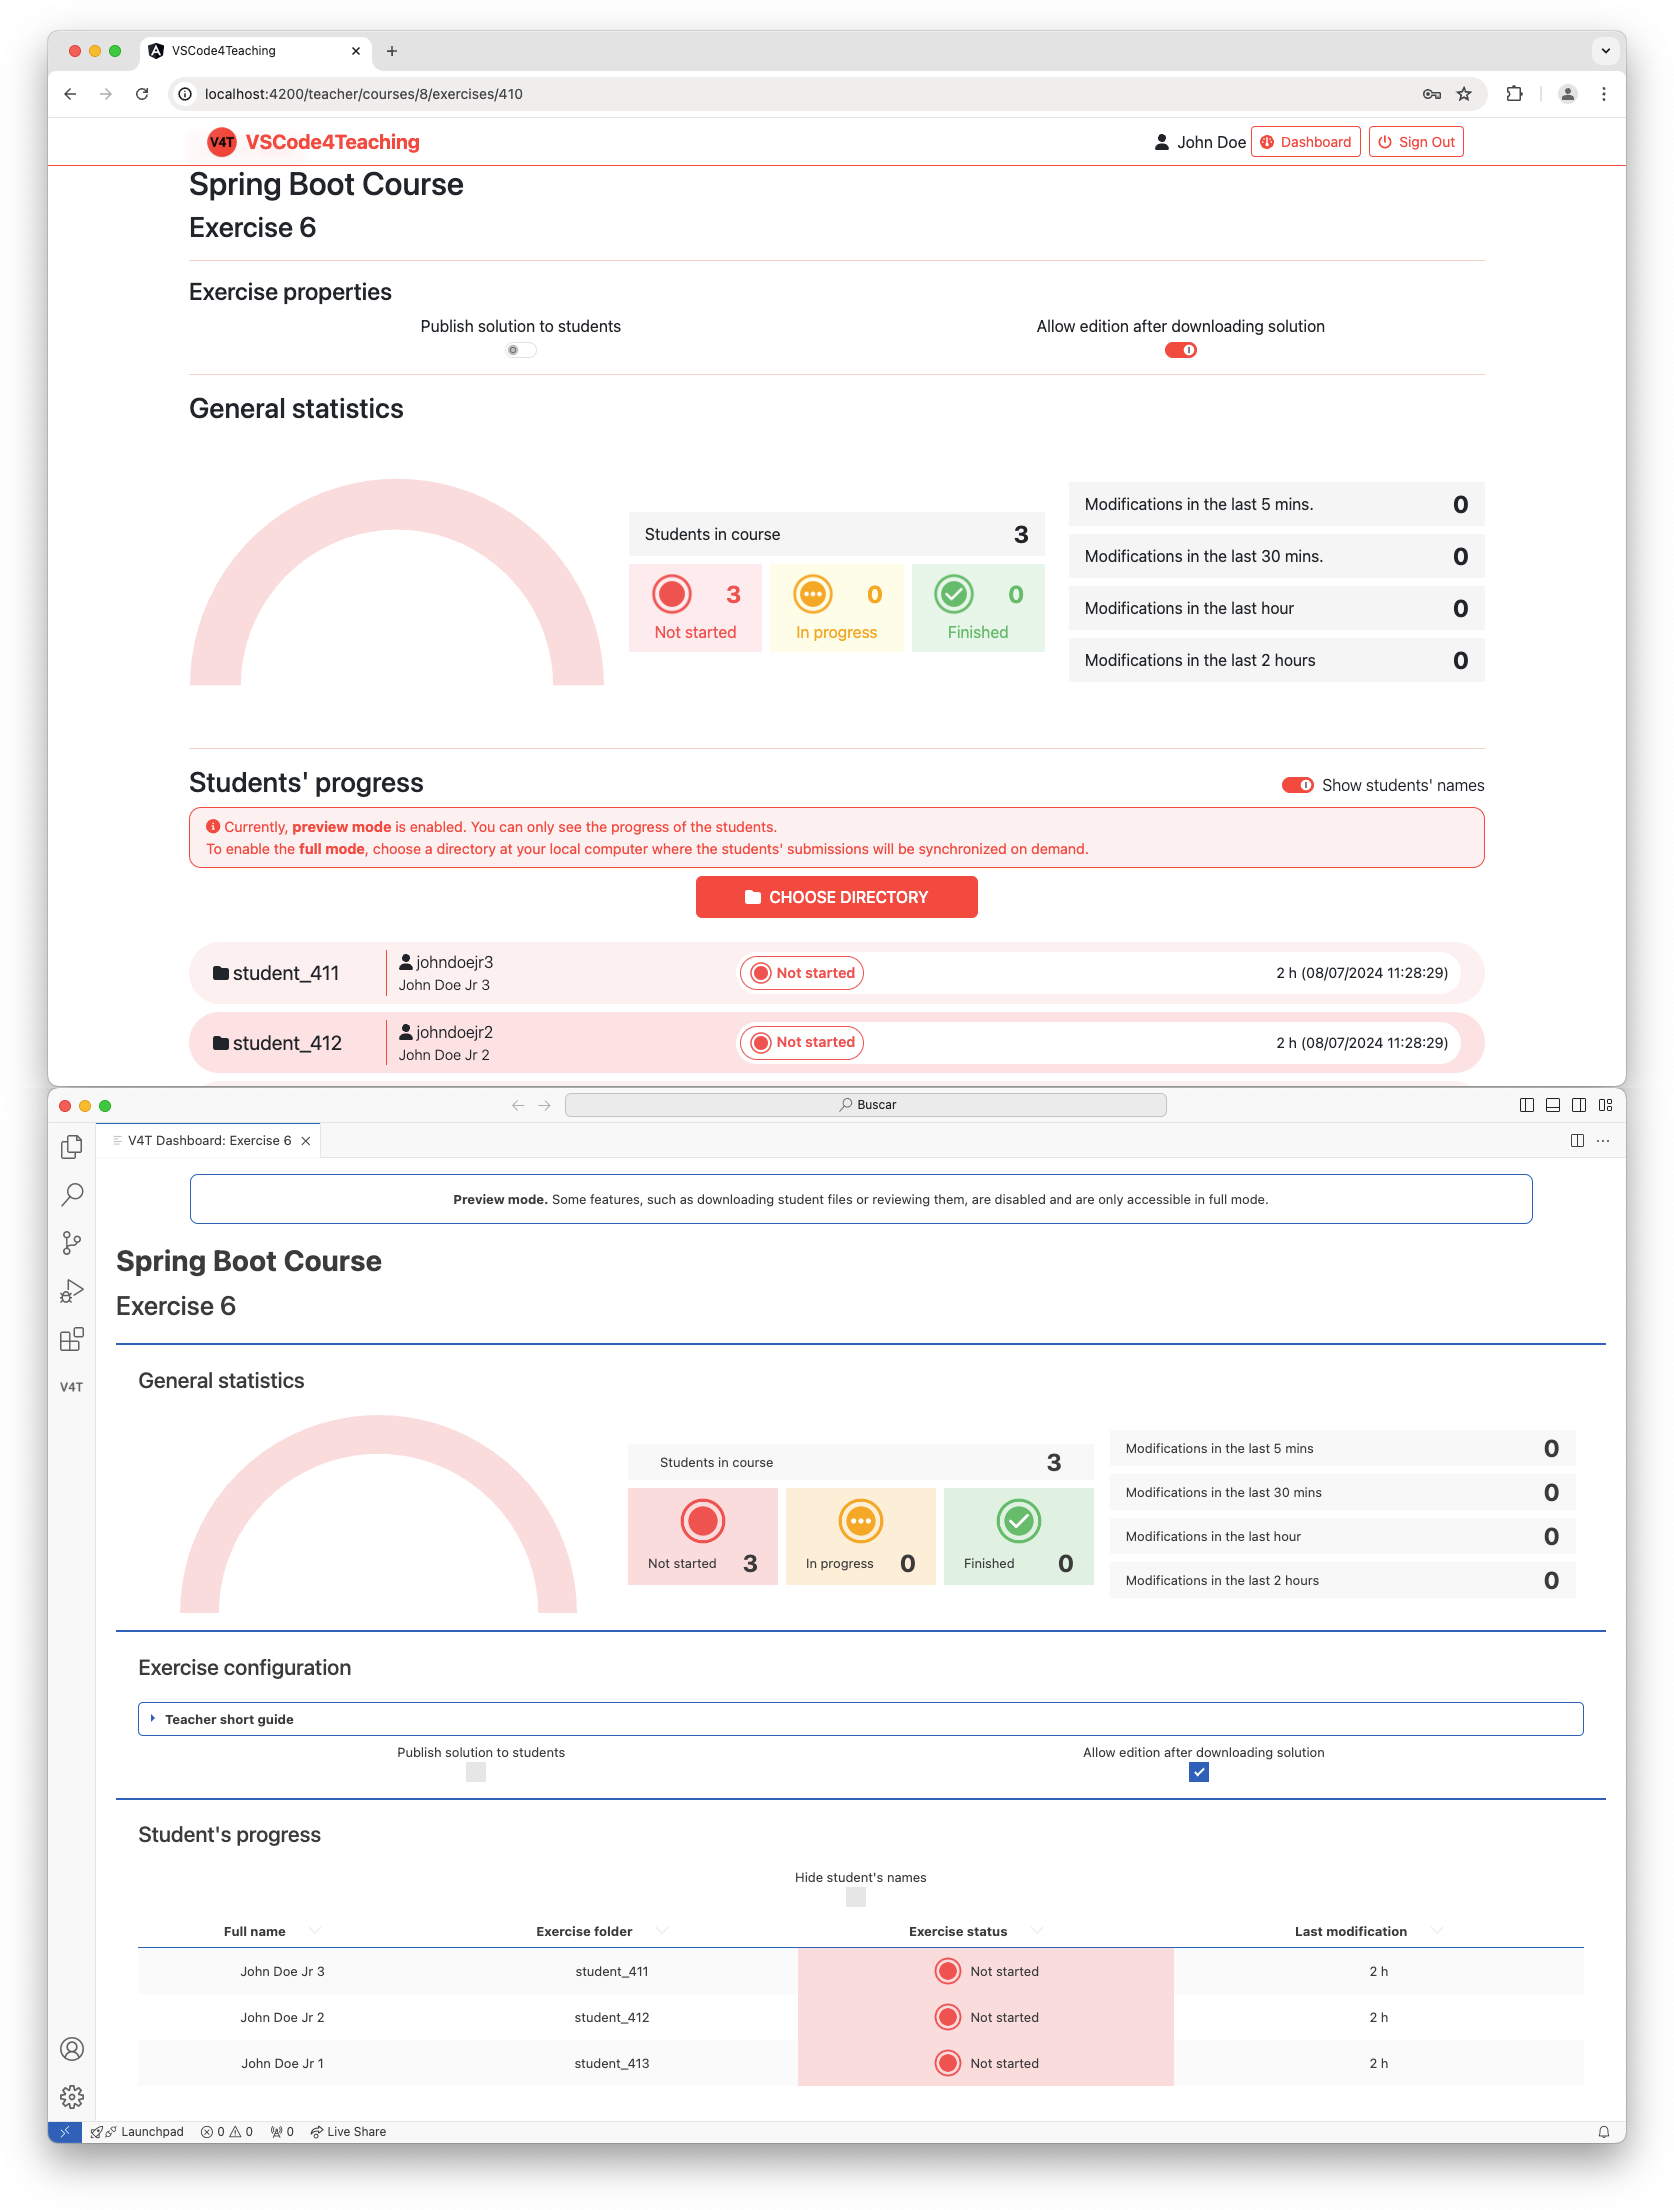
\includegraphics[width=\textwidth]{imagenes/utilizadas/4-3-implementacion/rn2-1.png}
    \caption{\textit{Dashboard} de un mismo ejercicio capturados a la vez en la aplicación web (arriba) y en la extensión para Visual Studio Code (abajo).}
    \label{fig:reqn2-1}
\end{figure}

\begin{figure}[ht!]
    \centering
    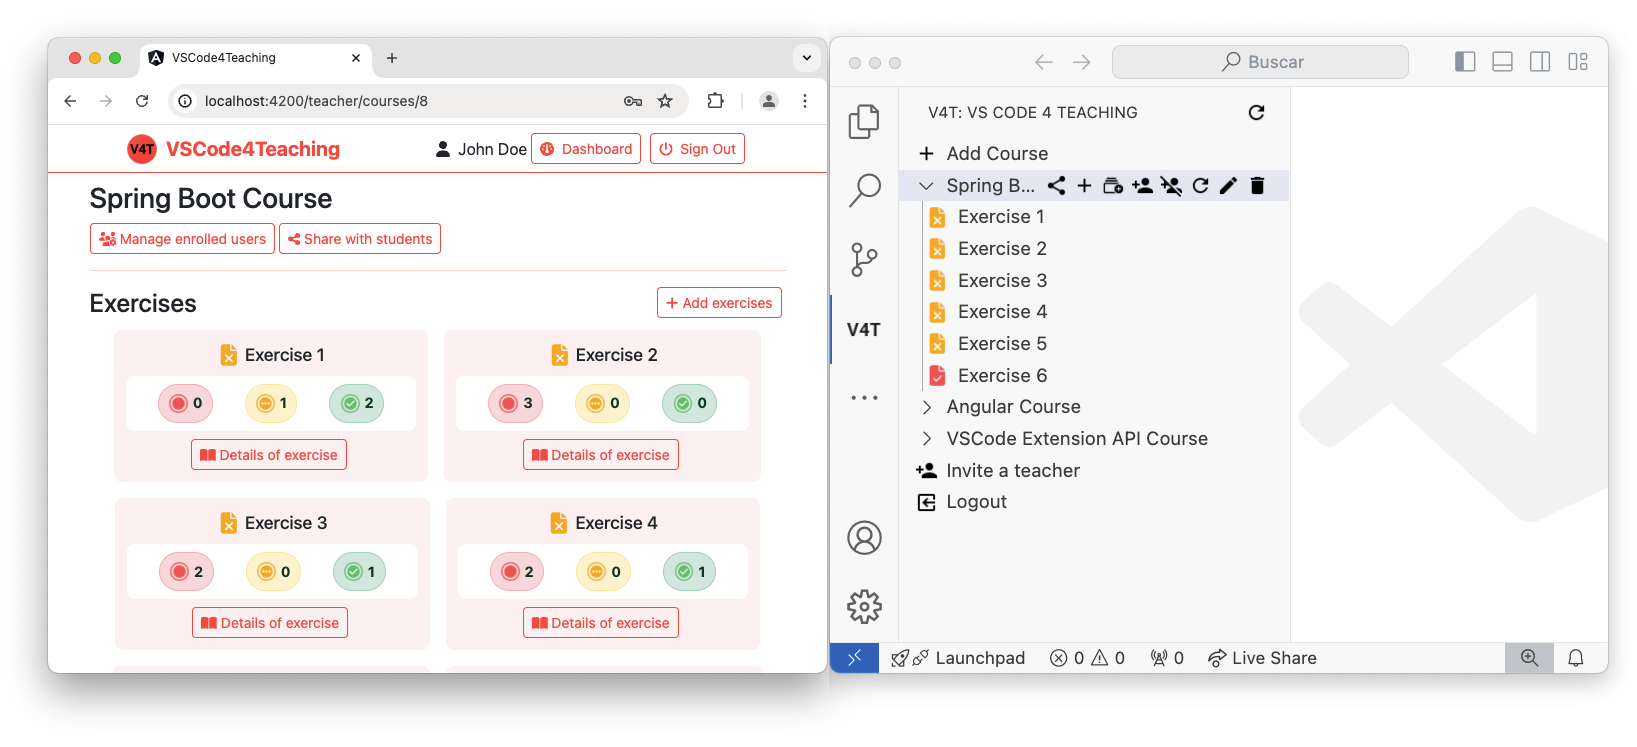
\includegraphics[width=\textwidth]{imagenes/utilizadas/4-3-implementacion/rn2-2.png}
    \caption{Comparativa entre los formatos empleados para mostrar a los docentes los ejercicios y configuraciones de las que disponen sus cursos.}
    \label{fig:reqn2-2}
\end{figure}
